% Template provided by LLNCS macro package for Springer Computer Science proceedings;
% Version 2.20 of 2017/10/04
%
\documentclass[runningheads]{llncs}
%
\usepackage{amsmath}
\usepackage{booktabs} % For pretty tables
\usepackage{caption} % For caption spacing
\usepackage{subcaption} % For sub-figures
\usepackage{graphicx}
\usepackage{pgfplots}
\usepackage[all]{nowidow}
\usepackage[utf8]{inputenc}
\usepackage{tikz}
\usetikzlibrary{er,positioning,bayesnet}
\usepackage{multicol}
\usepackage{algpseudocode,algorithm,algorithmicx}
\usepackage{minted}
\usepackage{hyperref}
\usepackage{enumitem}
\usepackage{blindtext}
\usepackage{graphicx}
\usepackage{comment}
\usepackage[inline]{enumitem} % Horizontal lists
% If you use the hyperref package, please uncomment the following line
% to display URLs in blue roman font according to Springer's eBook style:
% \renewcommand\UrlFont{\color{blue}\rmfamily}
\usepackage{lipsum}
\usepackage{mwe}
\usepackage{titlesec}
\usepackage{siunitx}
\captionsetup[table]{skip=7pt}
\renewcommand\paragraph{\@startsection{paragraph}{4}{\z@}%
   {-3.25ex\@plus -1ex \@minus -.2ex}%
   {1.5ex \@plus .2ex}%
   {\normalfont\normalsize\bfseries}}
\makeatother
\renewcommand{\labelitemii}{$\star$}
\renewcommand{\labelitemii}{$\cdot$}
\usepackage[
backend=biber,
style=alphabetic,
sorting=ynt
]{biblatex}
\addbibresource{refs.bib}
\graphicspath{ {./images/} }

\renewcommand{\algorithmicrequire}{\textbf{inputs:}}
\renewcommand{\algorithmicrequire}{\textbf{local variables:}}
\renewcommand{\algorithmicensure}{\textbf{return:}}

\setcounter{secnumdepth}{3}% Number up to \subsubsection

\newcommand{\card}[1]{\left\vert{#1}\right\vert}
\newcommand*\Let[2]{\State #1 $\gets$ #2}
\definecolor{blue}{HTML}{1F77B4}
\definecolor{orange}{HTML}{FF7F0E}
\definecolor{green}{HTML}{2CA02C}

\pgfplotsset{compat=1.14}

\renewcommand{\topfraction}{0.85}
\renewcommand{\bottomfraction}{0.85}
\renewcommand{\textfraction}{0.15}
\renewcommand{\floatpagefraction}{0.8}
\renewcommand{\textfraction}{0.1}
\setlength{\floatsep}{3pt plus 1pt minus 1pt}
\setlength{\textfloatsep}{3pt plus 1pt minus 1pt}
\setlength{\intextsep}{3pt plus 1pt minus 1pt}
\setlength{\abovecaptionskip}{2pt plus 1pt minus 1pt}

\begin{document}

\title{Human-Computer Interaction Final Report}
\author{Emme McCabe, Nicole Nigro, Anaïs Sarrazin}
\institute{Computer Science Department, Bowdoin College, Brunswick, Maine, USA}
%\email{ acsarraz@bowdoin.edu}\\}

\maketitle             

% Abstract
% A condensed version of the Introduction (optional)
\begin{abstract}

The digitization of restaurants has resulted in more and more restaurants offering online food ordering as well as the widespread use of major food delivery apps. However, the unique designs of these online food ordering platforms have rarely been studied in depth. We were interested in learning about user experiences accessing and navigating different online food ordering platforms. To explore this topic, we used qualitative and quantitative data from a user study with 8 participants. This user study asked those surveyed to complete comparable tasks on ePub, the online food ordering platform that we built, and Portland Pie, a local competitor. With this data, we were able to assess and compare the efficiencies and aesthetic qualities of the two designs. Our findings show that ePub’s design is more time efficient and straight-forward than Portland Pie’s. These results demonstrate how design aspects like how a menu is displayed or where a cart is located have a significant effect on user experience. We discuss the implications of this for the design of more efficient online food ordering platforms, which can hopefully help create optimal user experiences on these platforms.

\keywords{Design \and User Experience \and User Interface \and Online Food Ordering}
\end{abstract}

% Introduction
% An overview of what you did, briefly addressing the following points outlined in the report guidelines. 
\section{Introduction}

We wanted to develop a solution that would improve the quality of life for the Bowdoin Community. While brainstorming ideas, we became hungry and decided to go to the Pub. However, we were unable to call the Pub or quickly grab it since we were in the library. Currently, the only way to order from the pub is to physically go there in person or order ahead by calling in. In a survey conducted by BankMyCell, 75\%\ of millennials avoid phone calls as they can be time consuming, where 64\% of these people avoid talking on the phone because they don’t want to talk to whiny or slow people \cite{bankmycellwebsite}.  These are serious constraints that pose a problem of accessibility because the pub is generally the only food option open after dining hall hours on weekdays. We realized that Bowdoin \textit{needed} to give students a way to order food from the pub while a) not physically being there and b) without having to make a phone call. 

Members of the Bowdoin community who regularly get food from the pub will find our topic interesting because it offers a new, more efficient way to order food. This is particularly valuable for people who have time constraints and cannot afford being on hold when the Pub is serving customer orders real-time or waiting for their food to be ready. Our system allows them to order their food online (they don’t need to be at the pub) and pick it up when they are ready; no time is wasted waiting at the pub. Also, people who don’t like talking on the phone or interacting with people will find this topic useful because it reduces human to human interaction to a singular interaction: picking up food and paying for it. This topic has the potential to draw in new customers who might have avoided the pub in the past because there wasn’t a convenient way to order food.

To illustrate the need for a new type of ordering system, imagine an end user Bowdoin student, Louis, who wants a buffalo chicken wrap with his favorite side - fries. It is 8:30 PM on a Wednesday and he is working in the Roux center on a lab report for his ecology class due at 11:59 PM that same night. He is both pressed for time and does not want to talk to someone on the phone who will mishear his order. He decides to walk over to the Pub, and ends up not returning until an hour later due, which makes him even more stressed out. Imagine instead that he goes online to an ordering system to order his food, where he can visually see his order to ensure that it is correct, while also seeing the time at which it will be ready, 9 PM, as to avoid waiting for his food to be ready. After having spent 30 minutes working on his report, Louis runs over to the Pub to pay for and pick up his food which is ready and heads back to the Roux to eat his food and finish up his lab report with ample time. 

In this paper, we introduce a system called the ePub, and evaluate its impact on increasing the Bowdoin Student quality of life. The ePub is designed to facilitate the ordering process for customers of Jack Magee’s Pub, while increasing the overall experience. 

In Section 2, we first present the details of existing solutions that our work builds off of and their contributions. In Section 3, we provide an overview of the interface, along with our rationale for the design features we created. This includes discussing our usability testing done to inform our overall final design. In Section 4, we describe a summative evaluation of the work we pursued when timing participants on a particular task, by addressing the materials and procedure we used in conducting our user study. In Section 4, we discuss our results and describe a statistical test we used to compare the task times. Finally, we conclude with a section that provides an overview of our interface and features, and the main findings of our experimentation, as well as discuss what the implication of our findings have on the future of human-computer interaction in our domain. 

\section{Related Work}

Though our proposed solution serves a rather niche audience, that of the Bowdoin community, there are several large-scale solutions to the problem of inefficient food ordering that exist. In a survey conducted by Statista in 2018 \cite{statista}, the restaurant delivery services that were the most used in the United States were Seamless (GrubHub), Postmates, UberEats, DoorDash, and Ritual. Here we analyze three of our competitors that have been successful in this market. 

\subsection{Competitive Analysis \#1: Postmates}

\begin{figure*}[ht!]
    \centering
    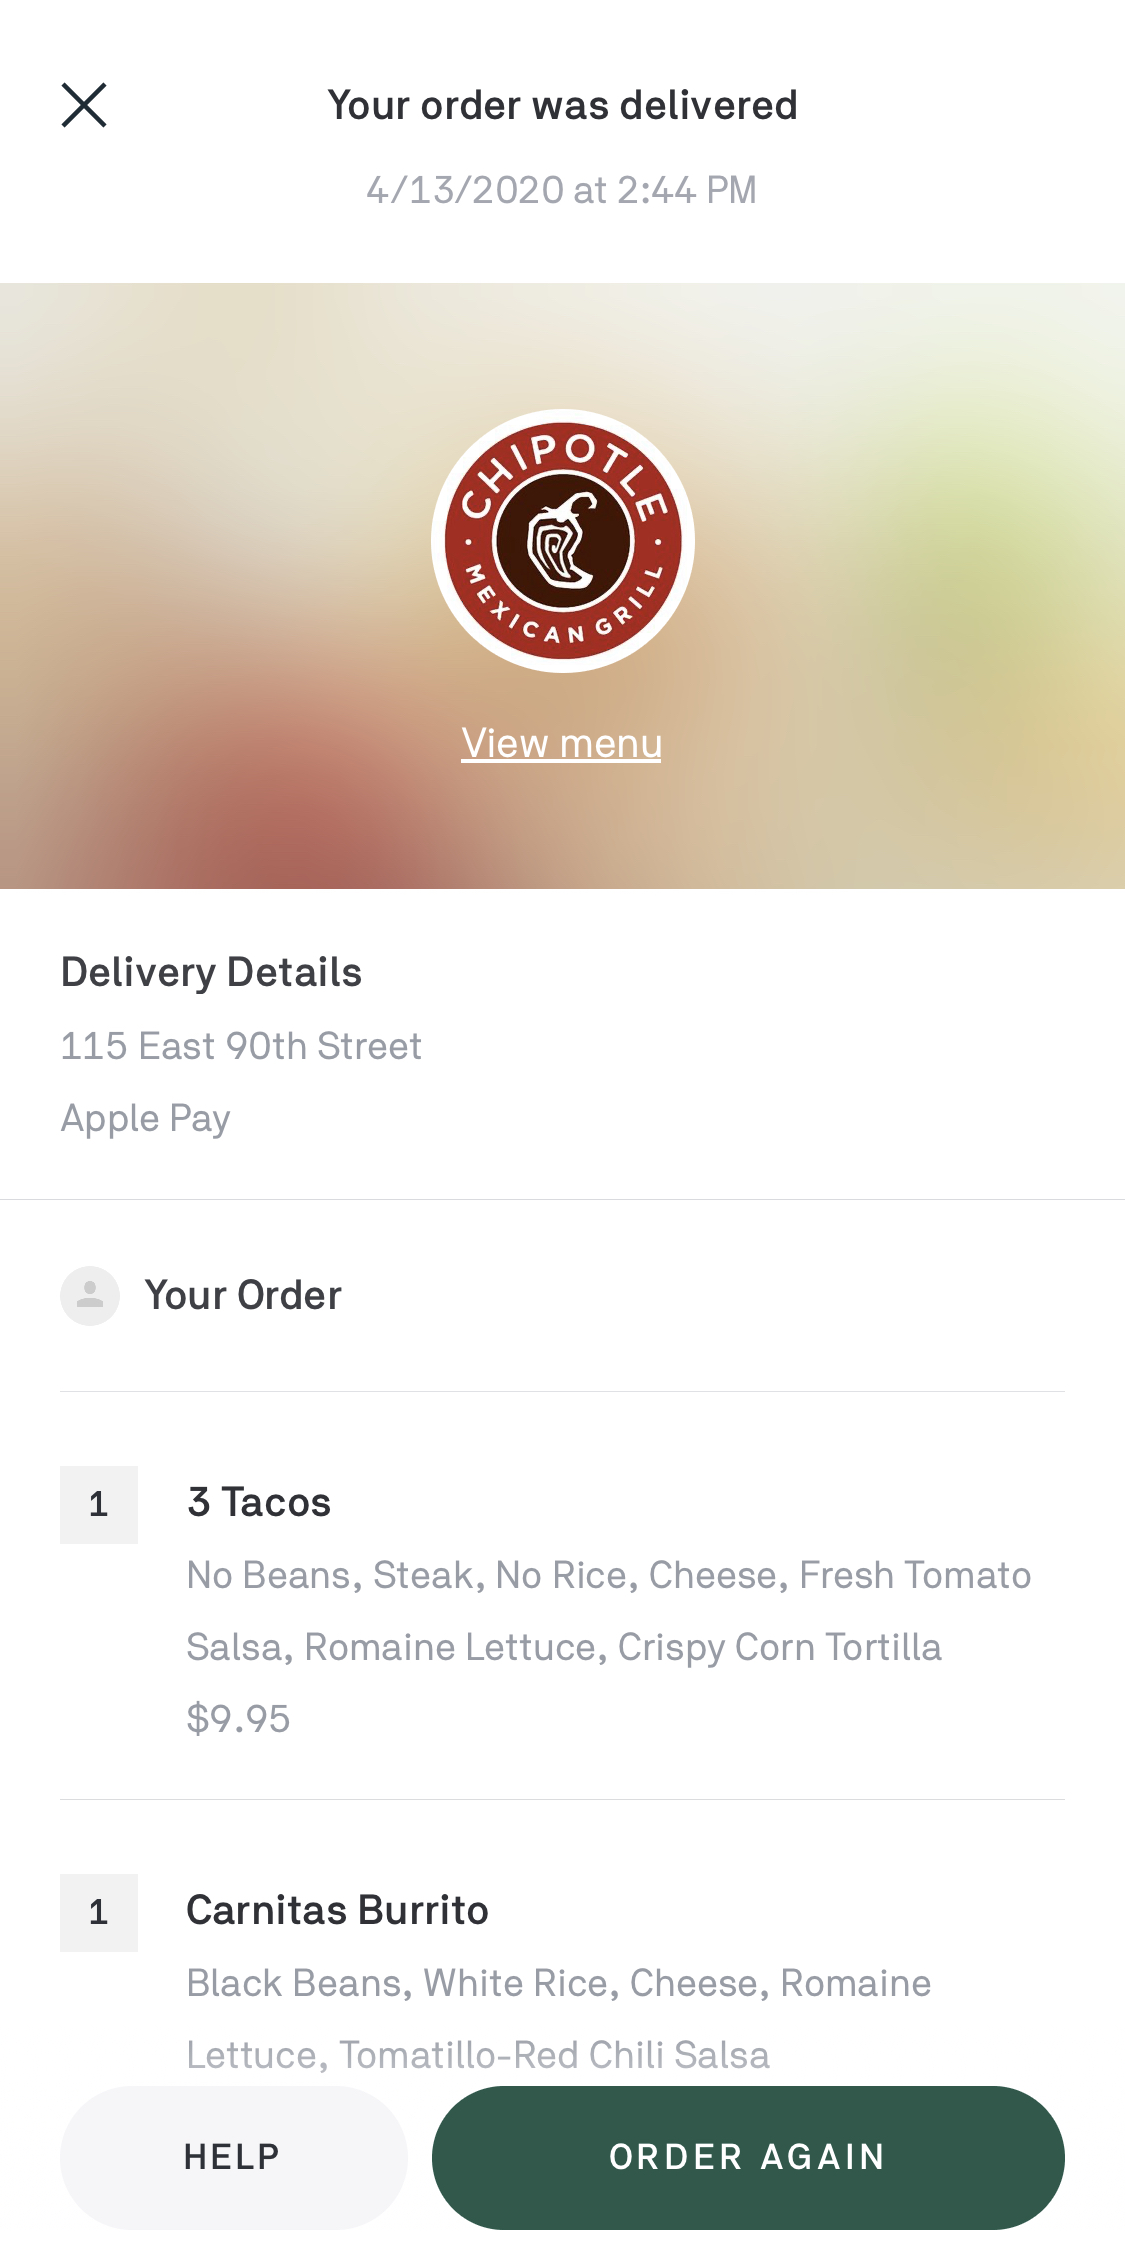
\includegraphics[width=.28\textwidth]{images/postmates-order-again.jpeg}\hfill
    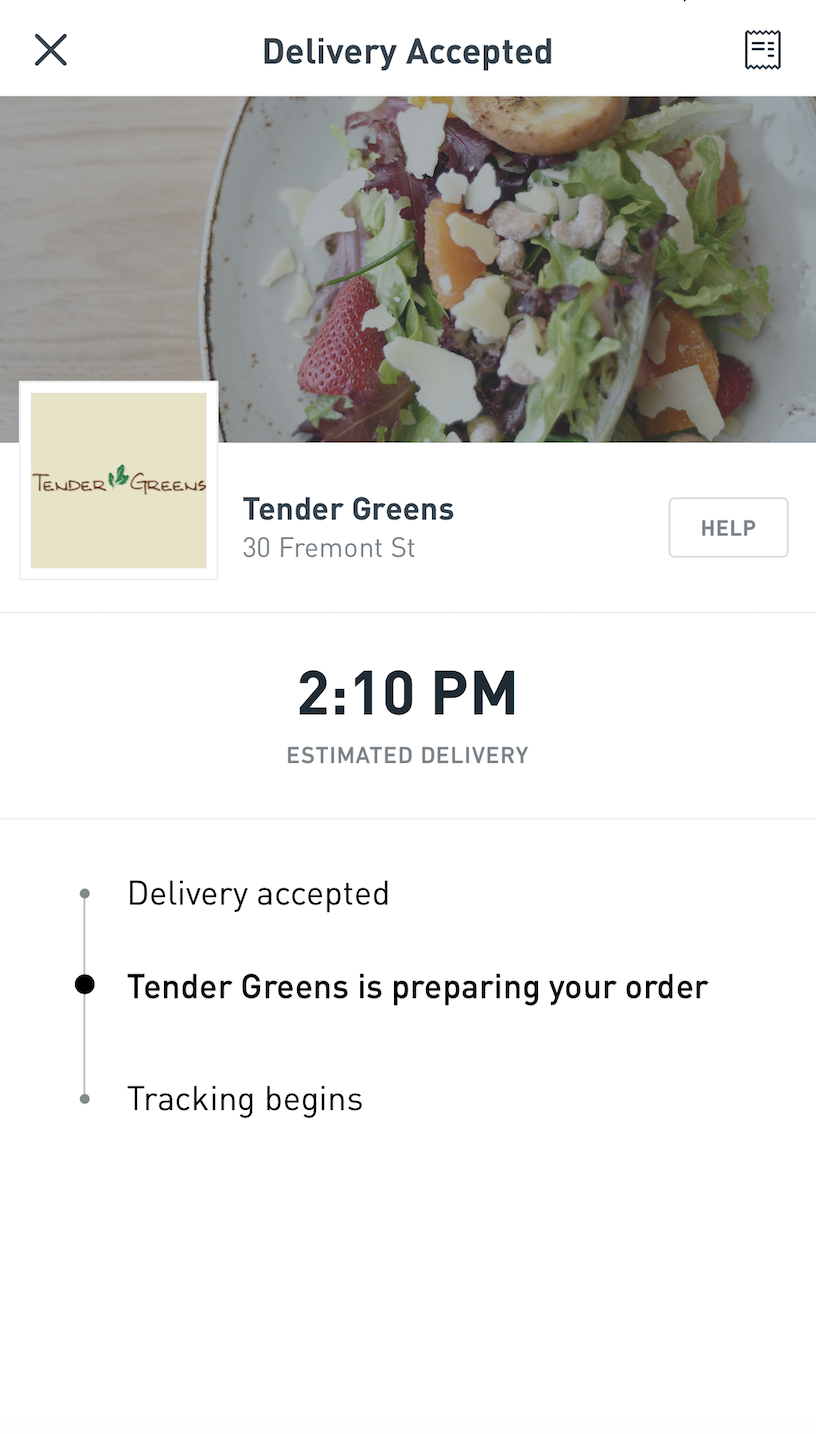
\includegraphics[width=.32\textwidth]{images/postmates-est-time-update.png}\hfill
    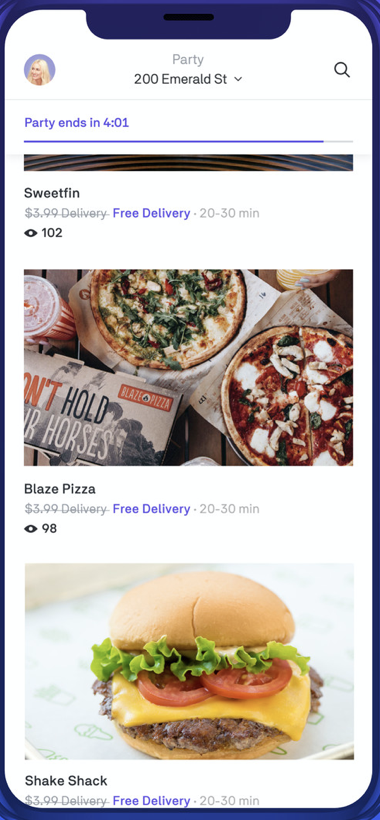
\includegraphics[width=.257\textwidth]{images/postmates-party-screen.jpg}
    \caption{(a) Order Again (b) Est. Delivery Time  (c) Postmates Party}
\end{figure*}

\noindent \textit{Order Again Button} \\
The ability to reorder past deliveries with the “Order Again” button provided by Postmates, as well as storing relevant customer data, is key in keeping customers. McKinsey \& Co. found that 80\% of customers rarely leave for another platform \cite{einstein}. \\ 

\noindent\textit{Notifications Updates } \\
This provides notification updates on the process of delivery, including when the order is placed, received, ready, picked up, and delivered. \\ 

\noindent\textit{Estimation of Delivery Time} \\
This gives the customer an idea of when the order will be delivered, so that they can prepare to be ready to grab their food from their door at this time. \\ 

\noindent\textit{Postmates Party} \\ 
Postmates Party gives the user real-time visibility on what other people around them are ordering. Restaurants that are being ordered frequently from are marked as “trending”. To join the “Party”, Postmates provides a button where the user can easily click and see what restaurants are trending and are given a window for how long these restaurants will trend for. This reduces time for delivery drivers as they pick up more food from a smaller pool of restaurants. \\ 

\noindent\textbf{Contribution #1} \\ 
Since ePub is focused on the efficient pickup aspect of the online food ordering service, it is extremely necessary for us to provide an order again button. As opposed to Postmates, our re-order button is conveniently placed right next to a past order, as soon as the customer has logged into their account, providing them with an easy way to order again. Also, since our system is primarily used on a computer, we did not see the integration of notification updates to be useful to the user. 

\subsection{Competitive Analysis \#2: UberEats}  

\begin{figure*}[ht!]
    \centering
    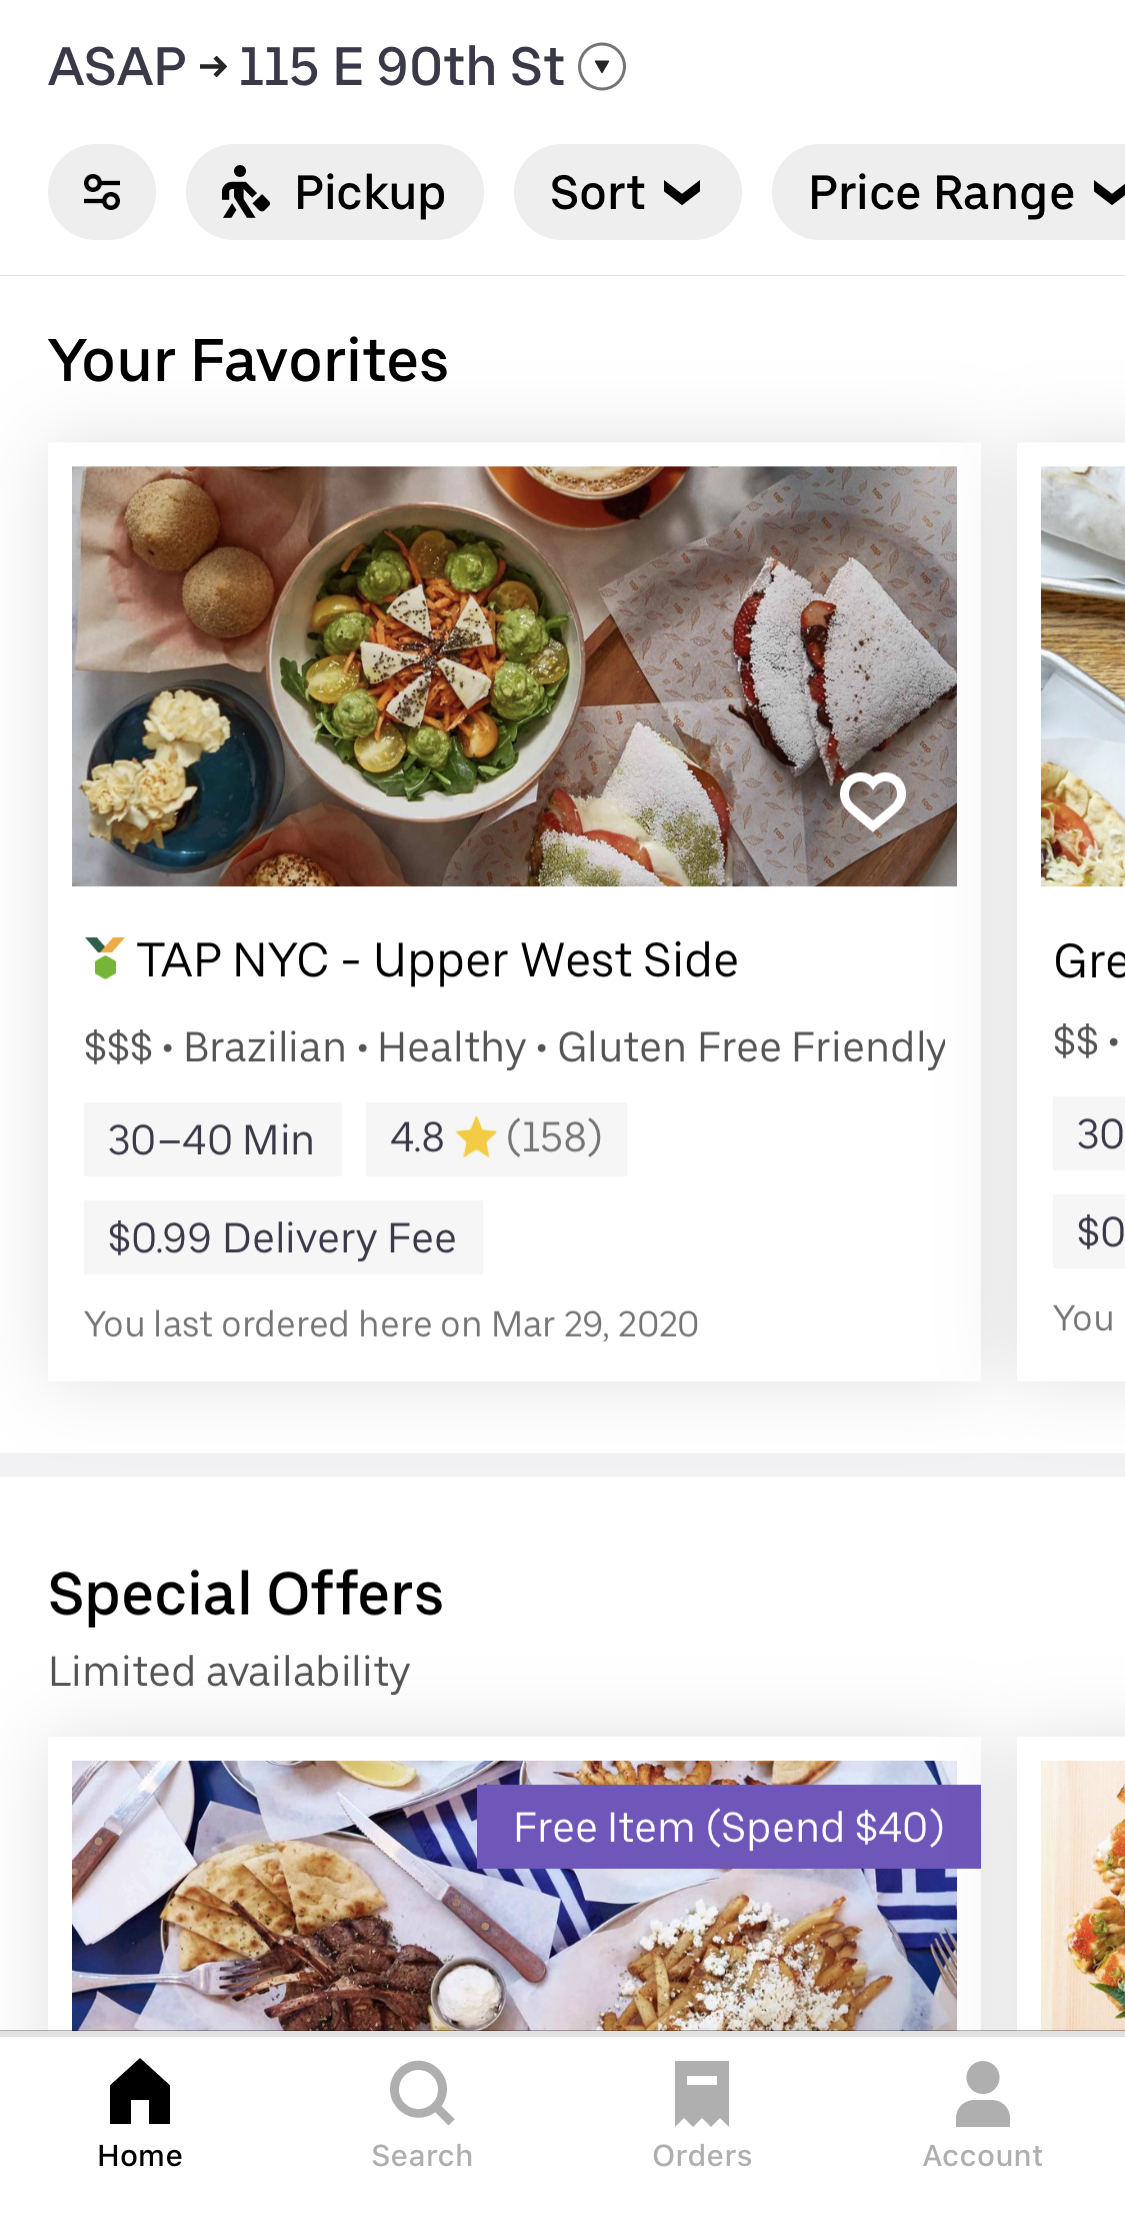
\includegraphics[width=.285\textwidth]{images/uber-eats-home.jpeg}\hfill
    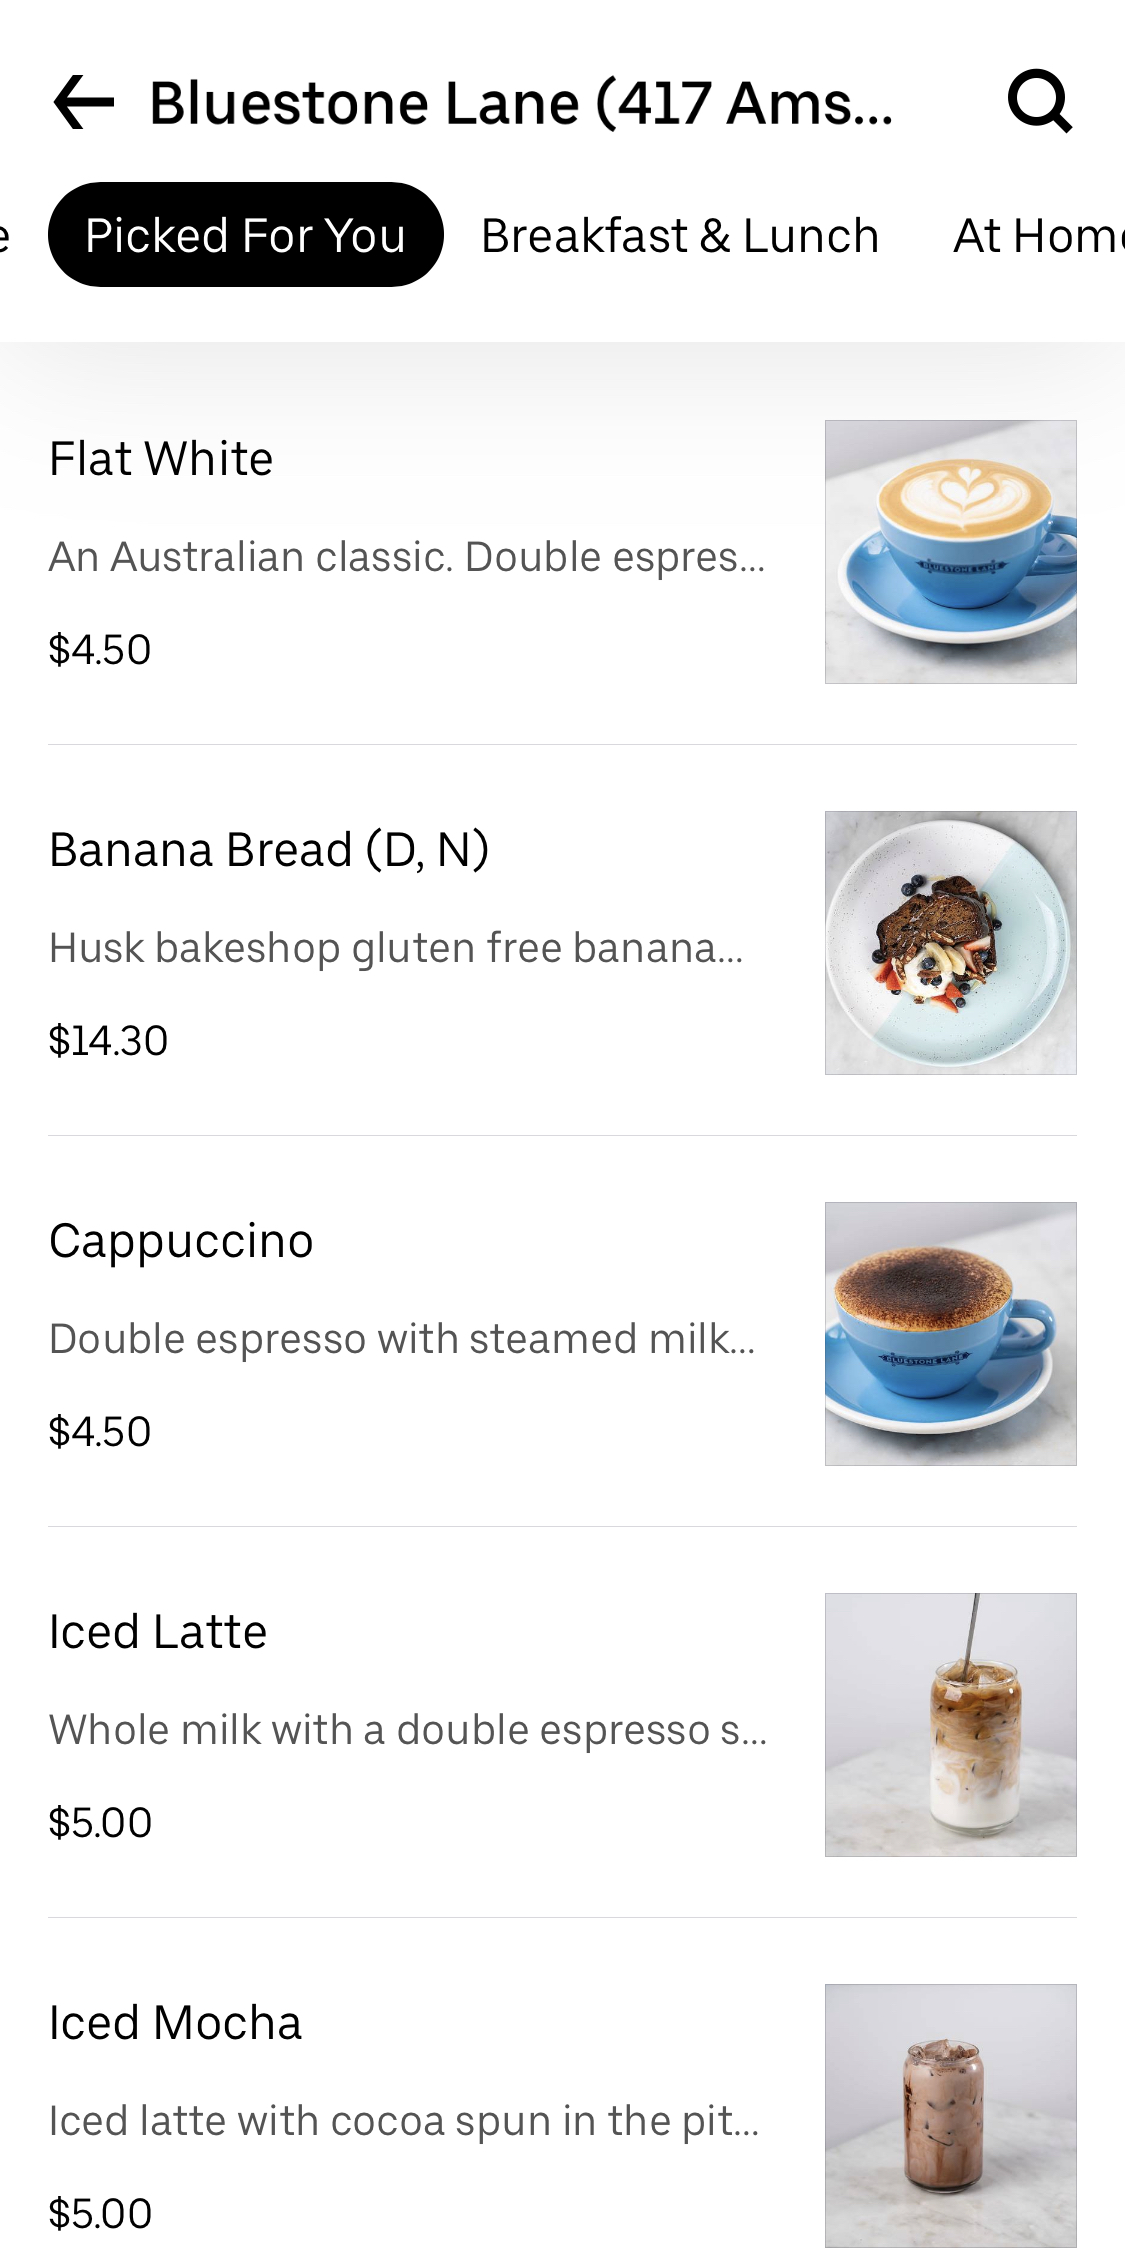
\includegraphics[width=.285\textwidth]{images/uber-eats-picked.jpeg}\hfill
    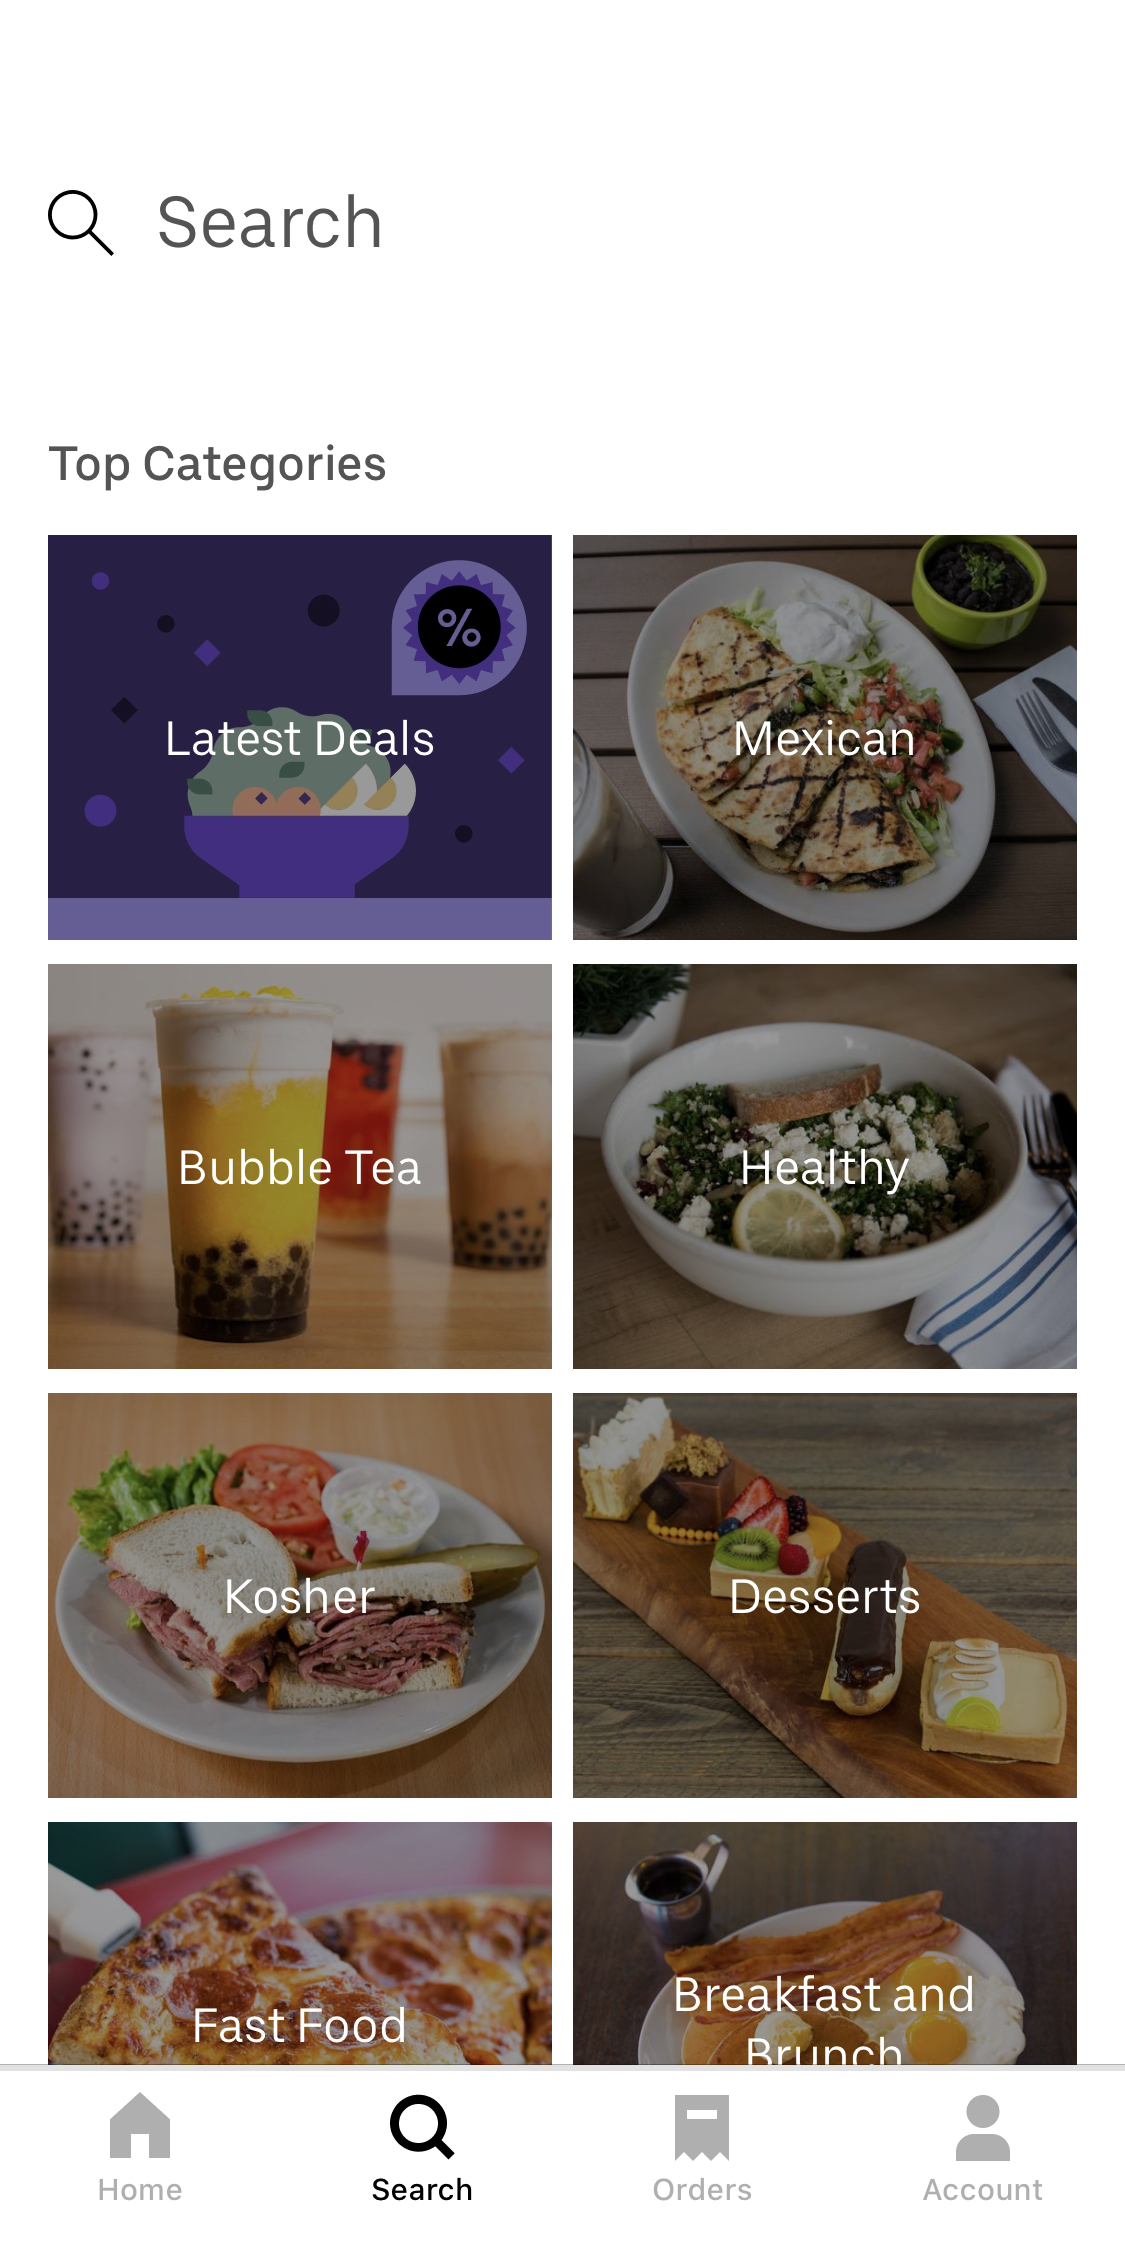
\includegraphics[width=.3\textwidth]{images/uber-eats-search.jpeg}
    \caption{(a) Home Screen    (b) Picked for You     (c) Search Options}
\end{figure*}

\noindent \textit{Simple and Aesthetic User Interface} \\
The app is extremely simplistic, with a white background and only holding essential options at the footer for the user (e.g. “Home”, “Search”, “Orders”, and “Account”). Most dishes are presented with an image to the right of the description. \\

\noindent\textit{Picked for You} \\ 
This option is available once the user has chosen the restaurant they want to order from. This is based off of the past orders the user has bought and provides incentive to the user to sign into their account to get this functionality. \\ 

\noindent\textit{Variety of Search Options} \\ 
Provides a large array of options on how the customer can choose to see the available options of restaurants and dishes available on the platform. It allows the customer to filter restaurants by the type of cuisine (e.g. vegan, Indian), particular dish preferred, price range (e.g. \$-\$\$\$), dietary restrictions, rating, and popularity. This system also allows them to sort the options in terms of their delivery preferences, such as delivery time and estimates, delivery fee, delivery or pickup.\\ 

\noindent\textbf{Contribution \#2} \\ 
In a similar way as Uber Eats, ePub provides a simple user interface for the customer to easily navigate the website and make orders quickly. However, since our system catered to only one restaurant, we didn’t feel the need to provide an abundance of search options. To continue with the simplicity of the UI, the system provides food options only by menu categories. \\

\subsection{Competitive Analysis \#3: DoorDash} 
\begin{figure*}[ht!]
    \centering
    %\includegraphics[width=.3\textwidth]{images/doordash-delight.png}\hfill
    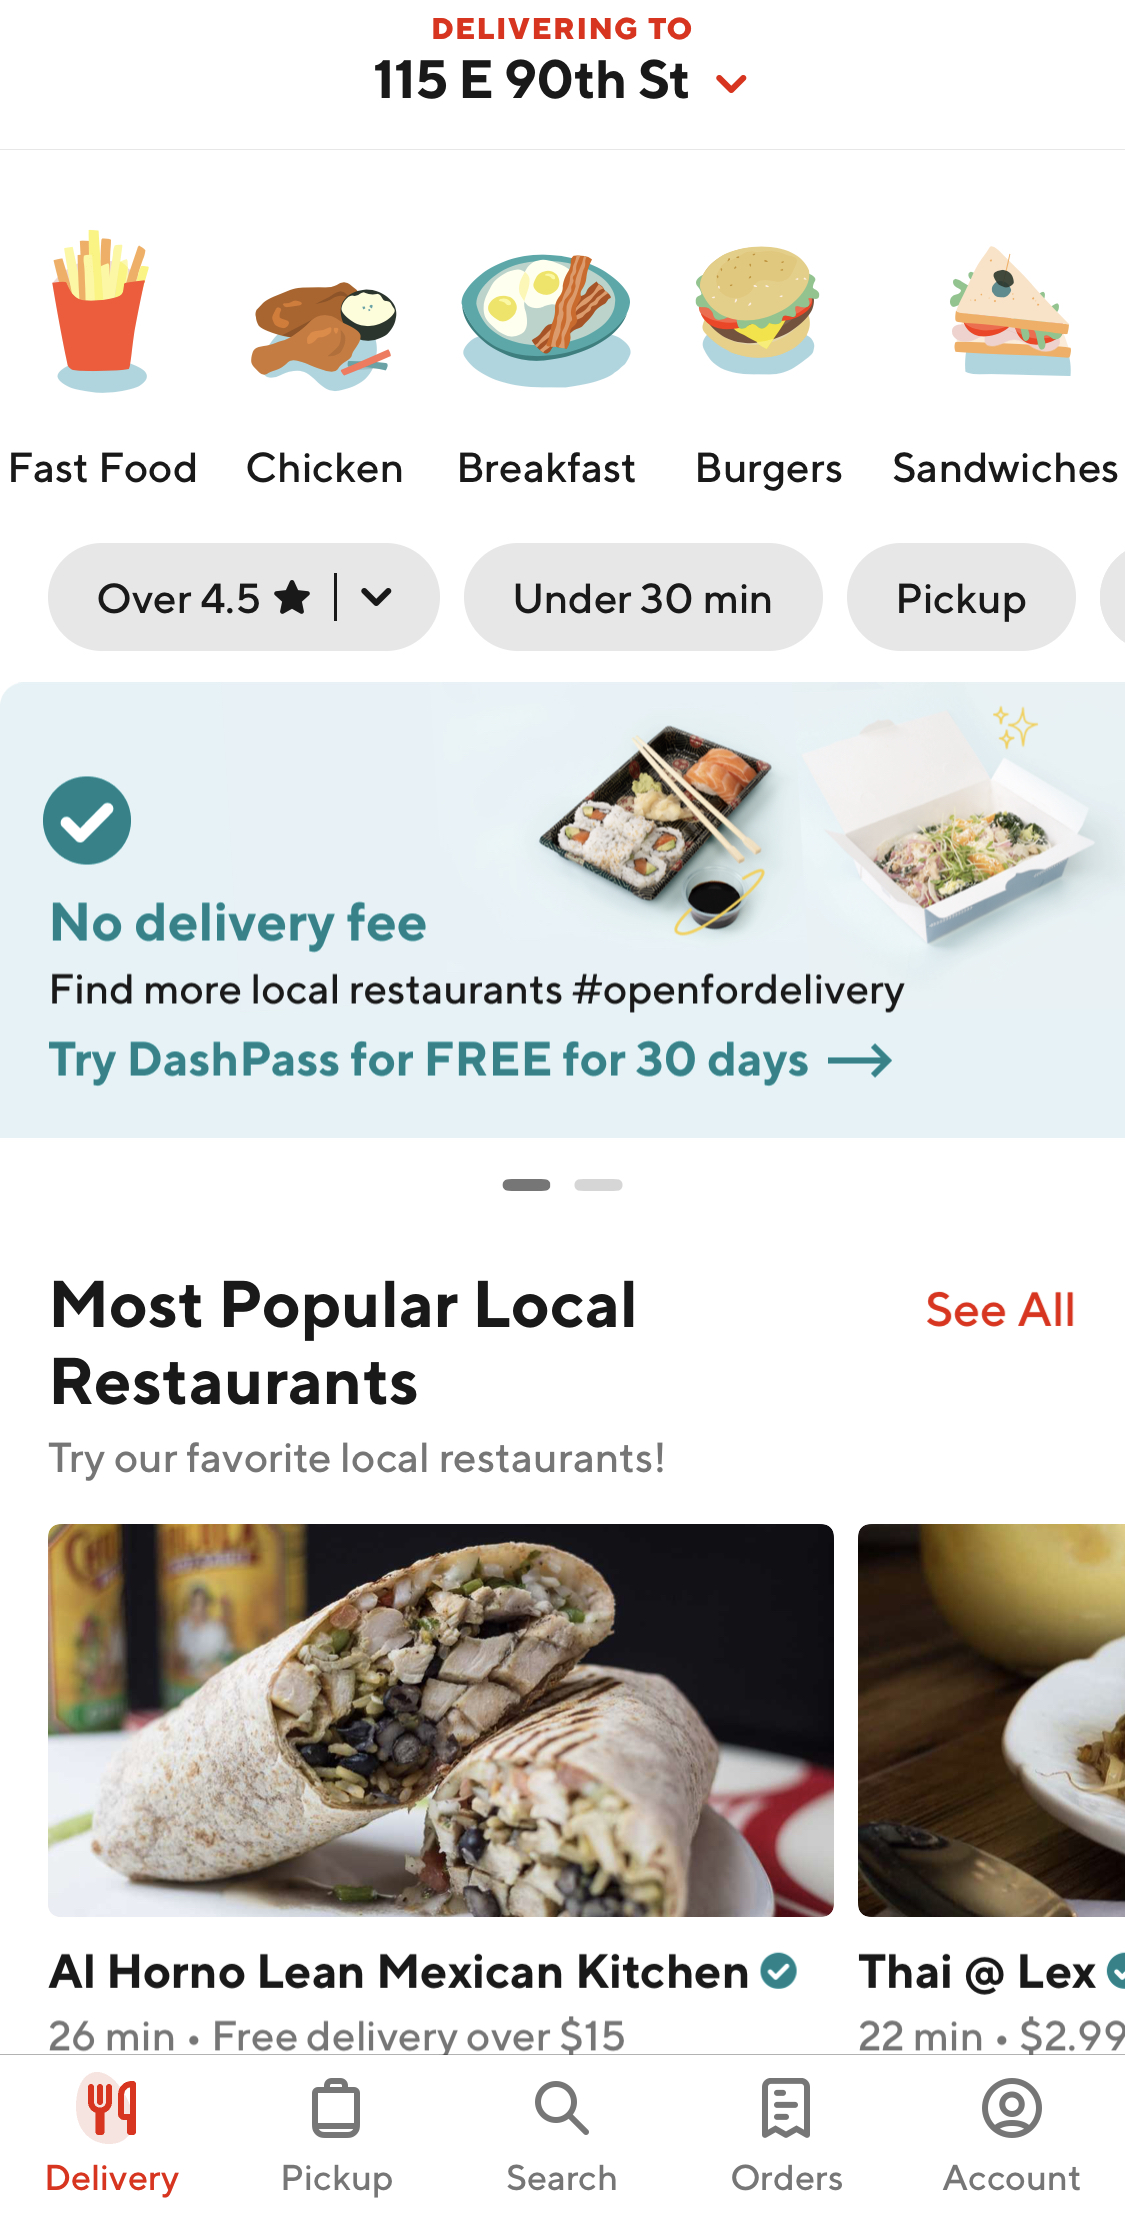
\includegraphics[width=.3\textwidth]{images/doordash-filters.jpeg}
    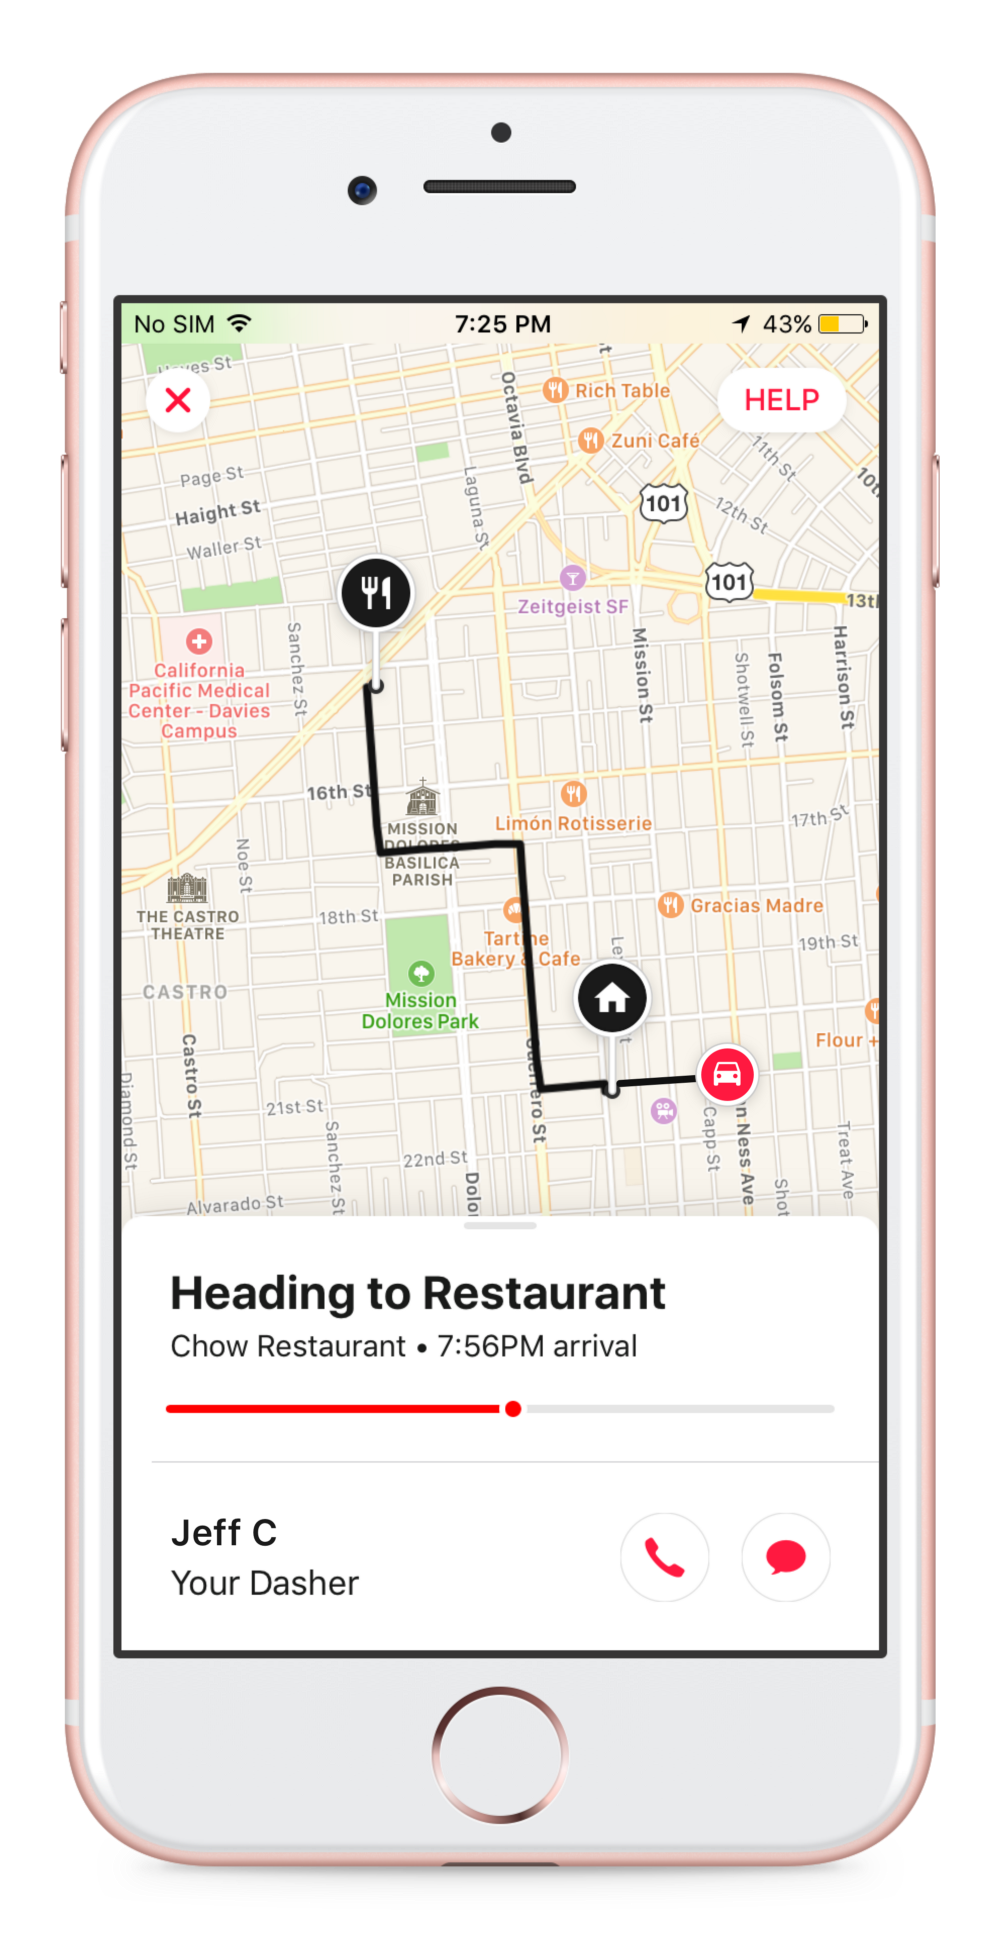
\includegraphics[width=.3\textwidth]{images/doordash-tracking.png}
    \caption{(a) Filter Optionsx (b)Tracking}
\end{figure*}
\noindent \textit{Easy to-use Filtering}\\
When opening the app, the user is directed to a main screen with different categories of filtering options. At the top of the screen, the user can choose to filter based on either the cuisine or type of meal or restaurant desired (e.g. Asian, Fast Food, Breakfast) by clicking on a recognizable icon (e.g. a fries icon for the Fast Food option). Below, it offers buttons for a variety of delivery preferences the customer could limit their searches to, such as “Under 30 min” and “Pickup”. The bottom sections offer catered categories based on the user’s location and past orders, including “Your Favorites” and “Fastest Near You”.\\

\noindent\textit{Real-Time Tracking} \\
This allows customers to see where their door dash driver is located in real-time.  \\

\noindent\textit{DoorDash Delight}\\
Created through the aggregation of customer feedback, Doordash’s “Delight Score” is a feature that rates the food delivery quality of different restaurants available from a scale of 1 to 10 \cite{ddelight}. This score allows customers to make better decisions on their food choices, while also helping them discover new restaurants. Additionally, customers can choose to filter their main page by highest to lowest “Delight Score.”\\

\noindent\textbf{Contribution \#3}\\
Similar to Uber Eats, DoorDash provides an abundance of filtering options. However, ePub is catered towards the Bowdoin community. As a result, the system only demonstrates the dishes based on the categories shown in the original menu of Jack Magee's Pub. This provides easy recognition by the customer when using our system. 

\section{Approach}

\subsection{Working Prototype \& Usability Testing}

\begin{figure}[H]
    \centering
    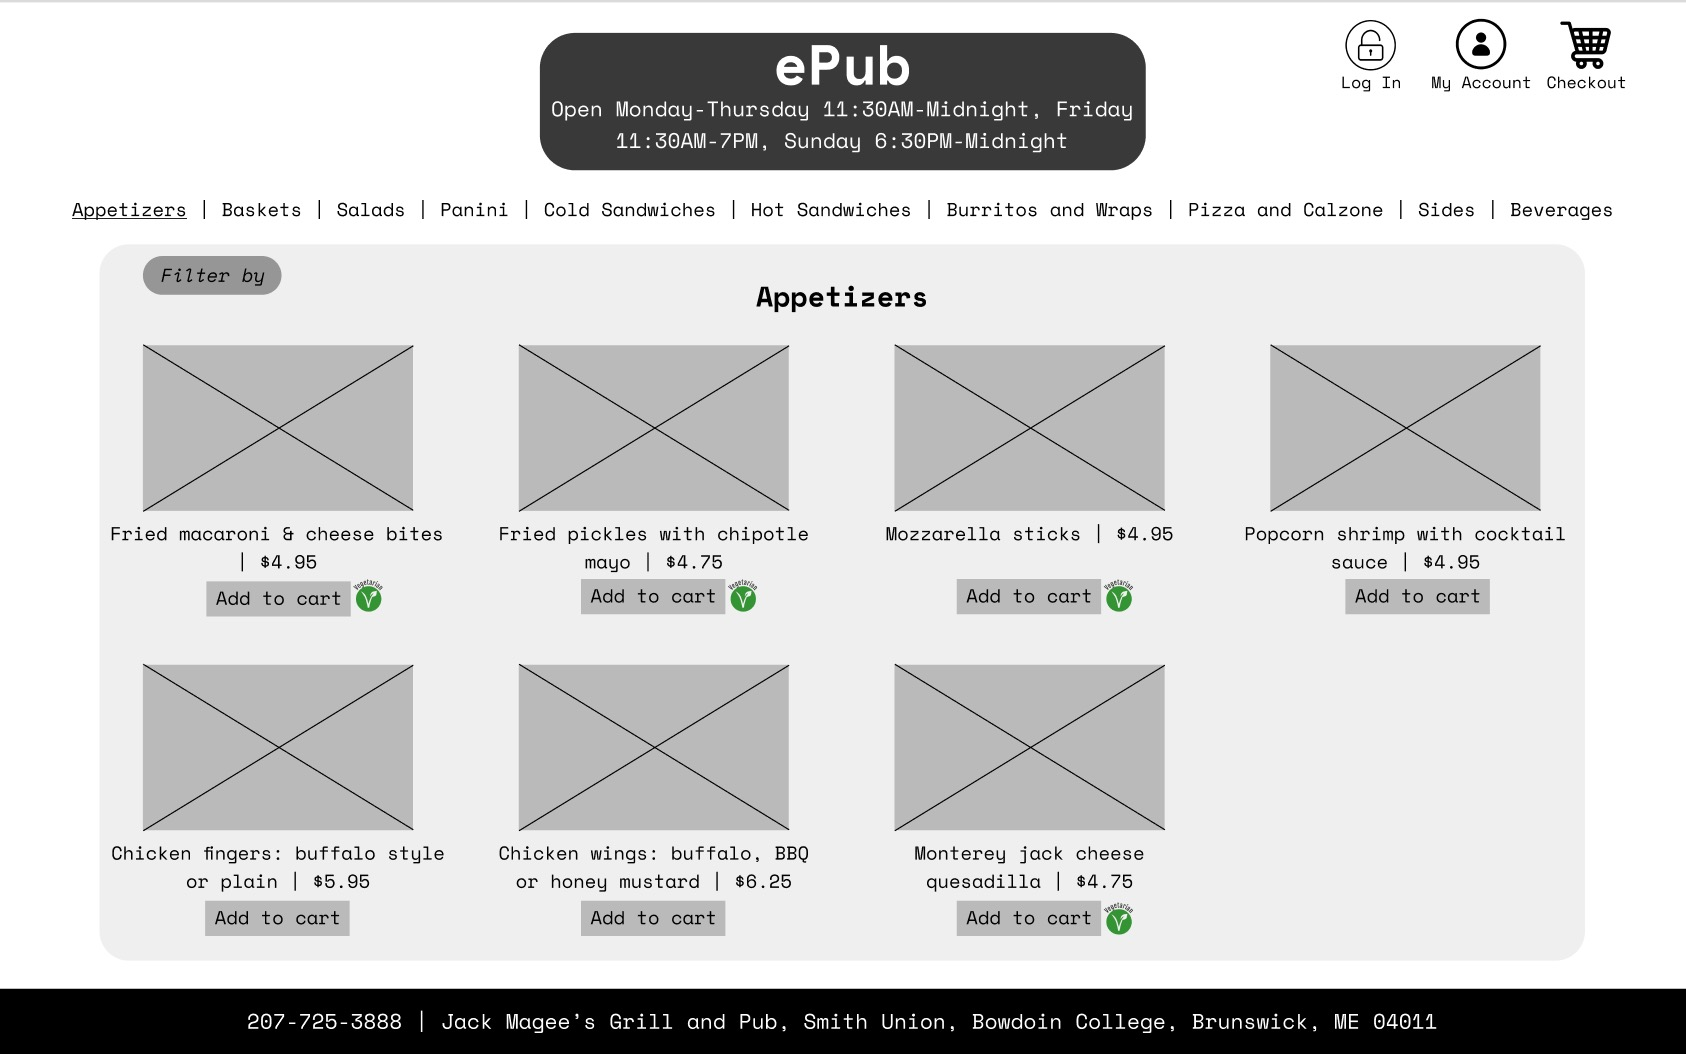
\includegraphics[width=13cm]{images/epub_design-nicole.jpeg}
    \caption{Initial Design for ePub}
\end{figure}

Prior to building our main prototype, we created an initial design for our system, that can be seen in Figure 1. Then, we identified the following user tasks that we were interested in testing: 
\begin{enumerate}
    \item As a returning customer, how would you reorder a specific item?
    \item How would you locate the ‘Chicken Pesto Panini’ and customize the order to add ‘Avocado’ and checkout? 
    \item Show me how you would get in contact if you made a mistake in your order. 
\end{enumerate}
Finally, we used these predefined tasks to gain feedback from our classmates about our current design representation. 

For our first task, classmates identified several ways to re-ordering a specific item from the website. As designers, we need to consider how users make decisions, based on both ease and speed. Classmates also assumed that there would be some sort of functionality on the ‘My Account’ page that would allow them to reorder a past item and suggested that we update our design to make this task more efficient and direct. 

For the second task, classmates completed this task quickly. We think this because they frequent the pub and are used to the menu display and process there, which we tried to recreate in our design. However, some of our classmates did have questions regarding how we would deal with customization add-ons that weren’t already available. This was important for us to consider as we build this website as if the user wants to add an ingredient, they need to be charged, but we cannot anticipate all the ingredients out there. 

Similarly to the second task, classmates completed this final task quickly. This is likely because the contact info (phone number, location) are highly visible in the footer of the website. Some classmates did provide design recommendations, such as adding a ‘Cancel Order’ button as well as removing the ‘Contact Us’ button, as it felt more like a button where you would go to get hired to work at the Pub, as opposed to contacting the Pub for help. 

\subsection{Overview of Features on Interface}  

Through the usability test feedback and through our own evaluations of our design using Nielsen’s Heuristics (link to appendix), we developed our interface with unique features that catered to our users’ needs. \\ 

\noindent \textit{Aesthetic \& Minimalist UI} \\ 
The system is very well laid out with only critical information displayed. Menu listings are streamlined and contain only the minimum information needed for a customer to make a decision on what to order: item name, price, whether or not it is vegetarian with the universally known vegetarian logo, and sometimes appealing pictures.\\ 

\noindent \textit{Recognizable Menu} \\
The menu on the system is organized like the Pub’s menu is organized on the Bowdoin website:  organized by different types of items (appetizers, salads), item name and price displayed on the same line with a bar in between. This feature was developed based on Nielsen’s first heuristic design of Match between system and the real world, which states that the system should be designed to speak the “users’ language, with words, phrases, and concepts familiar to the user.”  This verisimilitude makes the organization of items familiar and easily accessible, even to new users.  \\ 

\noindent \textit{Easy-to-Use Checkout}  \\ 
The add to cart functionality and checkout cart in the upper right icon are similar to popular e-commerce sites like Amazon, so the flow should be intuitive and familiar to users. Without having to go to a new page, the user is able to quickly look at their cart to see the items in their cart. \\

\noindent \textit{Reorder Capability}\\
When conducting our usability testing, classmates assumed that there would be some sort of functionality (e.g. see history button) on the ‘My Account’ page that would allow them to login to their account and reorder a past item. Through this assumption, we created a simple ‘Reorder’ button that makes it efficient for those who have logged in to their accounts to simply press on their past order.\\

\noindent \textit{Visible Documentation and Contact Information}\\
Since the process of placing an order at the Pub via ePub is very different from the already existing solutions, many first-time users may encounter difficulties as they will not know the steps they must take on the website to place an order and what responsibility they have once they place an order. In our initial inspecting process of our prototype design, we identified this to be a medium impact problem through the use of Nielsen’s heuristics, as this only affects users who can’t intuit how to use the site. However, this poses extreme repercussions for these types of users as it could prevent them from placing an order. As a result, we created a FAQ page to guide users on how to effectively use the website to order with ePub by outlining the steps to using ePub and answering common questions, such as where to pick up the food. Additionally, the highly visible footer holding contact information allows for easy contact when making errors, as seen during our usability testing stage by our classmates.\\

\section{Methods}
We asked 9 classmates, chosen by Professor Harmon, to participate in our user study and 4 did. We then asked 4 more Bowdoin students outside of the class to reach the user study minimum of 8 participants. This was a convenience sample--a type of non-probability sampling that involves the sample being drawn from the part of the population that is close to hand \cite{wikiconveniencesampling}. Convenience samplings are most useful for pilot testing, so the data we collected gives us some preliminary results about our product’s usability. However, this data is limiting because there is so little of it (small sample size) and the group is not representative of the various personas that would potentially use our product. In the future, we hope to conduct a full scale research project that has a diverse sample reflective of our potential user base.

We gathered our data individually and remotely, so we did not have control over our participant’s environment. We used a survey that we created on Google Forms to collect responses from participants. For each design (ePub and PortlandPie), we asked participants to upload screen recordings of them completing the task, report the times it took to complete the task (using a timer), and select 3 words from a word bank of  23 words that best described their experience with the design. Participants completed these surveys on their computers (which vary in model), but as a control, we asked them to use the same web browser when completing both tasks. We used Overleaf to compile a document with the instructions for the user study and embedded links to our website and survey. We sent this document to our participants via Slack message. The raw data from the survey was stored in a Google Sheets Spreadsheet.

Our independent variable was design type and our dependent variables were the time to complete the task and the words used to describe the design. We used a within-subjects design, which means that all participants are shown both conditions. For each design, we included instructions for tasks we wanted them to complete. We counterbalanced to prevent the effect of which design is shown first on the results by showing one group (4 participants) ePub first and the other group (4 participants) Portland Pie first.

For each design, we asked participants to start a screen recording and timer then click on the link to the given design. The ePub design task provided a link that took participants to our ePub site. Once there, we asked participants to find the Chicken Pesto Panini and add it to their cart (1 item in cart). Then, remove the Panini from their cart (empty cart). Lastly, we asked them to find a cheeseburger and add it to the cart (1 item in cart), then add a second cheeseburger to the cart (2 items in cart). Once they finished these tasks for ePub, we asked participants to stop their timers and screen recordings. The Portland Pie design task provided a link to the Portland Pie online ordering site. Then, we asked participants to select pickup and locate the Brunswick, ME location. Next, we asked participants to find the Downeast Buffalo Sandwich and add it to their order (1 item in cart). Then, remove that sandwich from the order (empty cart). Finally, we asked that they find the Casco Bay Calzone and add it to their cart (1 item in cart), then add another Calzone to the cart (2 items in cart). Once they completed these tasks for Portland Pie, we asked them to stop their timers and screen recordings. After completing the tasks for both designs, we asked participants to click on the link to our survey and fill it out. 

\section{Results}
In this section, we will evaluate variables of participants' task completion times and descriptive statistics on the aesthetic features of the two tasks. The tasks were counterbalanced, so that half of the participants completed ePub online ordering first, and the other half of the participants were presented with Portland Pie online ordering first. 

We had two hypotheses for our user study, with the variables $T_a$ representing the time to complete the task for ePub and $T_b$ representing the time to complete the task for Portland Pie. Our null hypothesis was $T_a$ $\approx$ $T_b$, which predicted that the only difference in performance between the two groups we are testing is completely due to chance. Our alternative hypothesis was $T_a$ $<$ $T_b$, which expected that the groups will complete the task for ePub quicker than the task for Portland Pie because the design for ePub is more efficient.

The users completed the task for the ePub design in 67.5 seconds on average. The fastest completion time was 17 seconds, while the slowest completion time was 110 seconds. The standard deviation of completion time using ePub was 27.15 seconds, suggesting a wide range of speed in the sampled participants. For the Portland Pie Online Ordering form, users completed the task in 118.63 seconds on average. The fastest completion time was 70 seconds, and the slowest completion time was 170 seconds. The standard deviation of completion time using the Portland Pie online ordering form was 33.31 seconds, also suggesting variance in the speed it took to complete the tasks in the sampled participants.The mean of ePub minus Portland Pie equals -51.13, which means that it takes nearly twice the time to complete the task with Portland Pie’s design (m=118.63) than it does for ePub’s design (m=67.5). \\

\begin{table}
\centering
\renewcommand{\arraystretch}{1.2}
\renewcommand{\tabcolsep}{4mm}
\begin{tabular}{|m{1.3cm}|m{3.2cm}|m{3.9cm}|}
\hline
\textbf{User ID} &\textbf{ePub Task Completion Time (seconds)} &\textbf{Portland Pie Task Completion Time (seconds)}\\ \hline
    IS &64 &123 \\ \hline
    NA &17 &77 \\ \hline
    KL &110 &170 \\ \hline
    CL &88 &120 \\ \hline
    SD &63 &116 \\ \hline
    BP &78 &150 \\ \hline
    LS &68 &123 \\ \hline
    BI &52 &70 \\ \hline
\end{tabular}
\caption{Task Completion Times}
\vspace{-4mm}
\end{table}

We did a paired sample t-test of task completion times for the 2 designs to assess the statistical significance of our data. There was significant average difference between ePub and Portland Pie task completion times ($t_7$=8.2763, p $<$ 0.0001). The two-tailed p-value is less than 0.0001--this difference is extremely statistically significant. The lower the p-value, the lower the probability of obtaining a result like the one that would be observed if the null hypothesis were true \cite{ttest}. This low p-value increases support for our alternative hypothesis and decreases support for our null hypothesis.

The most selected word used to describe the ePub design was straight-forward (75\%) followed by the words organized (25\%), usable (25\%), effortless (25\%), simplistic (25\%), efficient (25\%) and intuitive (25\%). The 6 most selected words to describe the Portland Pie design were confusing (38\%), unattractive (38\%), time-consuming (25\%), attractive (25\%), customizable (25\%), and straight-forward (25\%). 25\% of surveyed users thought Portland Pie’s design was straight-forward, while 75\% thought ePub was straight-forward. 38\% of surveyed users would describe Portland Pie’s design as confusing, while none thought that ePub was confusing.

As seen in the table 1, there was an interesting contrast in participant NA’s completion times: they completed the task for ePub in just 17 seconds, but took nearly 4.53 times as long to complete Portland Pie’s task (in 77 seconds). Also, participant BI was the only one to use the words quick and easy to describe Portland Pie’s design, and they completed it that task the fastest of all those surveyed (in 70 seconds). Participants BP and NA both chose time-consuming as a word to describe the Portland Pie design: BP had the second slowest task completion time for the Portland Pie task while NA had the second fastest completion time.

\section{Discussion}
Our results affirm our alternative hypothesis that the groups will complete the task for ePub quicker than the task for Portland Pie ($T_a$ $<$ $T_b$). We hypothesized that this would be the case because the design for ePub is more efficient; however, our design aesthetic qualities results indicate that this could be because ePub’s design is more straight-forward than Portland Pie. The original motivation for the design was to create a seamless platform for Bowdoin students to place orders at the Pub, which would improve their time efficiency and order accuracy. In addition, we wanted the design’s organization and aesthetic simplicity to guide users to complete orders in minimal time.

The wide range in task completion time can also be attributed to a relatively small sample size. The participants, however, are all presumed Computer Science majors/minors and associated college students who frequently interact with eCommerce websites.

With the closing of on-campus classes and a transition to remote learning, we were limited in backend testing functionality. If campus life and Jack Magee’s Pub and Grill remained open, the team could have carried out far more extensive experimental user tests, in both B2C and B2B forums. These limitations do not undermine our findings, although testing the order pickup process would have greatly improved the effectiveness of the system we built.

The online ordering interface system, ePub, effectively removes the human-human interaction, by forging a human-computer interaction that eliminates errors in the transaction process. The findings of our study allowed us to understand users’ priorities in aesthetic features, in addition to time efficiency in an online ordering system. The domain of B2C food pickup and delivery products similar to ePub, has grown exponentially in recent years and especially as an essential business during the months of global pandemic.

In future integration of ePub with Jack Magee’s Pub and Grill, user testing will have to continue. The interesting areas students will need to research will be centered around efficiency over in-person, or phone ordering. The same laddering studies we conducted at the beginning of our process will be useful in comparing the efficacy of ePub over other restaurant options in Brunswick, ME. Technical aspects that users will need to test include up to date refreshes of daily specials, order accuracy and pickup time estimates. Furthermore, an interesting study could also include a delivery component to ePub. As students return to campus, with uncertainty about safety and social distancing, the ePub system could provide a framework for more no-contact systems at the College.

Based on the user study, we deduced that college students value a streamlined online ordering process. When compared to Portland Pie’s online ordering system, ePub allowed users to complete comparable tasks faster. We can conclude that online ordering systems designed for college students should serve the customer’s needs, compared to similar B2C software platforms that are very general. The creation of a proprietary system such as ePub, allows Jack Magee’s Pub and Grill to have customized information and menu items displayed on the website. The platform will require student assistance for site maintenance or a simple backend interface for Pub employees. In addition to task completion time, students also favored the aesthetic qualities of ePub compared with Portland Pie. The implications of this finding should guide online ordering designs that prioritize organization, simplicity and straight-forward.

\section{Appendix}

\subsection{User Study Full Questionnaire: \textit{(see raw data folder)}}
\begin{flushleft}
\begin{enumerate}
    \item What is your name?
    \item How long did it take you to complete Task A? (Either ePub or Portland Pie)
    \item Upload your screen recording of Task A.
    \item Now that you have completed Task A, select three words from the word bank below that best describe your experience using the given design: (random word order)
    \item How long did it take you to complete Task B?
    \item Upload your screen recording of Task B.
    \item Now that you have completed Task B, select three words from the word bank below that best describe your experience using the given design: (random word order)
\end{enumerate}
\end{flushleft}

\subsection{Paired $t$ test results}
\begin{flushleft}
\textbf{P value and statistical significance:}\\
The two-tailed P value is less than 0.0001\\
By conventional criteria, this difference is considered to be extremely statistically significant. \newline

\textbf{Confidence Interval:}\\
The mean of ePub minus Portland Pie equals -51.13\\
95\% confidence interval of this difference: From -65.73 to -36.52 \newline

\textbf{Intermediate values used in calculations:}\\
t = 8.2763 \\
df = 7 \\
standard error of difference = 6.177
\end{flushleft}

\section{Acknowledgements}
We would like to thank Professor Harmon for guiding us with our project, helping with technical components, and offering insightful feedback. \\
\\
We also want to thank the 8 participants of our user study for their time and responses. The data we collected from them allowed us to complete a thorough analysis of our design's efficiency and aesthetic qualities.\\
\\
We want to acknowledge the LLNCS macro package for Springer Computer Science Proceedings \textit{(see llncs.cls)}, which provided the template we used to compile this report in Overleaf.\\
\\
Lastly, we appreciate Blackrock Digital LLC for granting us permission to use their Bootstrap templates \textit{(see LICENSE in project code)}. Those templates were an important foundation for our final ePub product.

\section{Bibliography}
\printbibliography
%\bibliographystyle{plain}
%\bibliography{refs}
\end{document}